\graphicspath{ {FutureWork/Images/} }


\chapter{Future Work}
\label{cha:futureWork}

\section{Introduction}
In this chapter 

Normalisation
Mapping Disease Codes
Distributed
RNN


\section{Generalization}




\section{Distributed Word2Vec}

MapReduce


\section{Classification Patients}

As mentioned in section \ref{sec:word2vec}, a trained 2-layer neural network can be placed before another neural network and function as a lookup table. In this section, we discuss a possible neural network which allows us to further investigate the effectiveness of our word2vec approach to classify patients.

\subsection{Problem Definition}

The medical history of a patient is seen as a time series with as datapoints an EHR. Based on the time series, we want to classify it into different disease trajectories. A patient who is classified into a specific disease trajectory, can be treated more specifically. \\

The medical data of multiple patients is a $3$ dimensional tensor, see figure \ref{fig:rnnData}. This data structure is the input structure for a neural network.

\begin{figure}[H]
	\centering
	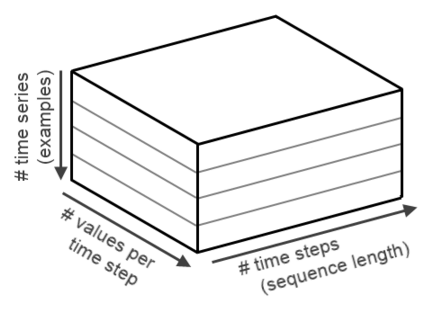
\includegraphics[width=8cm]{rnnData.png}
	\caption{Overview of the data structure for medical data with a time aspect.}
	\label{fig:rnnData}
\end{figure} 

Medical data has some problems which we will discuss.\\
It often consists of long time periods. This means there could be a long range of dependencies between events. In the context of training neural networks, this can cause a problem known as the vanishing gradient problem. \\
Patients don't have regular intervals in their medical data. The irregular intervals need to be transformed to regular intervals otherwise the time aspect won't be consistent throughout the data. \\
The standardization of the attributes needs to be taken into account. Preferably some sort of normalization should be applied as well. \\
Medical data has a high dimensionality. A lot of parameters need to be taken into account to retrieve accurate results. This causes the well known problem: Curse of Dimensionality. It causes the data to be sparse and therefore, more data is needed. Especially in medical data where outliers are important. 


\subsection{Approach}

Vanishing gradient
padding
Word2Vec standardization
Recurrent -> high dimension


\subsection{Neural Network}

We mentioned the reasons on why we choose a Long Short Term Memory (LSTM) approach as a recurrent neural network solution. In this section we explain in more detail why LSTM handles the vanishing problem and long-term dependencies. \\

First we shortly repeat the structure of a neural network in figure \ref{fig:nnStructure}. We see the input, different layers with their perceptrons, and $\sigma$ as the activation function. 

\begin{figure}[H]
	\centering
	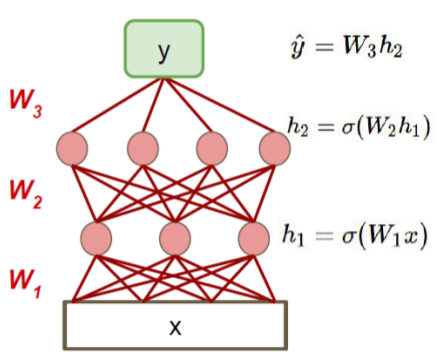
\includegraphics[width=8cm]{nnStructure.png}
	\caption{A general structure of a neural network.}
	\label{fig:nnStructure}
\end{figure} 

\subsubsection{Recurrent Neural Network}




\subsubsection{LSTM}


http://deeplearning4j.org/usingrnns

Supervised Sequence Labelling with Recurrent Neural
Networks

Phenotyping of Clinical Time Series with LSTM
Recurrent Neural Networks

IMEC Technical talk by Jaak Simm

Missing covariate data in medical research: To impute
is better than to ignore


Recurrent Neural Networks for Missing or
Asynchronous Data

Development of a Database of Health Insurance
Claims: Standardization of Disease Classifications and
Anonymous Record Linkage

Machine Learning Based Missing Value Imputation
Method for Clinical Dataset

Modeling Temporal Dependencies in High-
Dimensional Sequences: Application to Polyphonic
Music Generation and Transcription

Long short-term memory neural network for traffic
speed prediction using remote microwave sensor data


Noisy Time Series Prediction using a Recurrent Neural
Network and Grammatical Inference

Neural Networks for Time Series Processing
Constructing a Non-Linear Model with Neural
Networks for Workload Characterization



http://colah.github.io/posts/2015-08-Understanding-
LSTMs

A Critical Review of Recurrent Neural Networks
for Sequence Learning

Bidirectional Recurrent Neural Networks
Optimization of Hidden Markov Models and Neural
Networks


LONG SHORT-TERM MEMORY

LSTM: A Search Space Odyssey

\section{Conclusion}
The final section of the chapter gives an overview of the important results
of this chapter. This implies that the introductory chapter and the
concluding chapter don't need a conclusion.



%%% Local Variables: 
%%% mode: latex
%%% TeX-master: "thesis"
%%% End: 
